%! suppress = MissingImport
%! suppress = MissingLabel
%! suppress = LineBreak

% CLI args https://tex.stackexchange.com/a/1501
\newif\ifhandout
\input{flags}

%! suppress = MissingLabel
%! suppress = DocumentclassNotInRoot
%! suppress = DiscouragedUseOfDef

% * Make friends tikz & colors
%   https://en.wikibooks.org/wiki/LaTeX/Colors
% * To enable vertical top alignment globally
%   https://tex.stackexchange.com/questions/9889/positioning-content-at-the-top-of-a-beamer-slide-by-default
% * Set handout from CLI
%   https://tex.stackexchange.com/a/1501
\ifhandout
\documentclass[usenames, dvipsnames, handout]{beamer} % https://tex.stackexchange.com/questions/224091/beamer-how-to-disable-pause-temporarily
\else
\documentclass[usenames, dvipsnames]{beamer}
\fi
% ------------------------------------------------

% Graphics
\usepackage{color}
\usepackage{tabularx}
\usepackage{tikz}
% https://tikz.dev/tikz-graphs
\usetikzlibrary{positioning, shapes.geometric, arrows, automata, graphs}
\tikzset{
    expr/.style={ellipse, draw=gray!60, fill=gray!5, very thick, minimum size=7mm, yshift=0.7cm},
    hexpr/.style={ellipse, draw=gray!60, fill=blue!15, very thick, minimum size=7mm, yshift=0.7cm},
    stmt/.style={rectangle, draw=gray!60, fill=gray!5, very thick, minimum size=5mm, yshift=0.7cm},
    decl/.style={rectangle, draw=blue!60, fill=gray!5, very thick, minimum size=5mm, yshift=0.7cm},
    hdecl/.style={rectangle, draw=blue!60, fill=blue!15, very thick, minimum size=5mm, yshift=0.7cm},
    subtree/.style={shape border rotate=90, isosceles triangle, draw=gray!60, fill=gray!5, very thick, minimum size=5mm, yshift=0.0cm},
}
\usepackage{blkarray}
\usepackage{graphicx}
\usepackage{forest} % https://tex.stackexchange.com/questions/198405/how-to-change-the-color-of-subtrees-in-tikz-qtree
% ------------------------------------------------

% Math
\usepackage{amsmath, amsfonts}
\usepackage{amssymb}
\usepackage{proof}
\usepackage{mathrsfs}
% Crossed-out symbols
% https://tex.stackexchange.com/questions/75525/how-to-write-crossed-out-math-in-latex
\usepackage[makeroom]{cancel}
\usepackage{mathtools}
% ------------------------------------------------

% Additional font sizes
% https://www.overleaf.com/learn/latex/Questions/How_do_I_adjust_the_font_size%3F
\usepackage{moresize}
% Additional colors
% https://www.overleaf.com/learn/latex/Using_colours_in_LaTeX
\usepackage{xcolor}
% Textual math symbols
\usepackage{textcomp}
% ------------------------------------------------

% Language
\usepackage[utf8] {inputenc}
\usepackage[T2A] {fontenc}
\usepackage[english, russian] {babel}
\usepackage{indentfirst, verbatim}
\usetikzlibrary{cd, babel}
% ------------------------------------------------

% Fonts: https://sites.math.washington.edu/~reu/docs/latex_symbols.pdf
\usepackage{stmaryrd}
\usepackage{cmbright}
\usepackage{wasysym}
\usepackage[weather]{ifsym} % https://tex.stackexchange.com/questions/100424/how-to-use-the-ifsym-package
% https://tex.stackexchange.com/questions/615300/pdflatex-builtin-glyph-names-is-empty
\pdfmapline{=dictsym DictSym <dictsym.pfb}
\pdfmapline{=pigpen <pigpen.pfa}
\usepackage{dictsym}
% ------------------------------------------------

% Code
% * Needs -shell-escape build flag
%   https://tex.stackexchange.com/questions/99475/how-to-invoke-latex-with-the-shell-escape-flag-in-texstudio-former-texmakerx
% * Set build directory
%   https://tex.stackexchange.com/questions/339931/latex-minted-package-using-custom-output-directory-build
\usepackage{minted}
\setminted{xleftmargin=\parindent, autogobble, escapeinside=\#\#}
% ------------------------------------------------

% Template
\usetheme{CambridgeUS}
\usecolortheme{dolphin}
% https://tex.stackexchange.com/questions/231439/beamer-how-to-make-font-larger-for-page-numbers
\setbeamerfont{headline}{size=\scriptsize}
\setbeamerfont{footline}{size=\scriptsize}
% Remove heddline
% https://tex.stackexchange.com/questions/33146/how-could-i-remove-a-header-in-a-beamer-presentation
%\setbeamertemplate{headline}{}
% Slide sizes
% https://tex.stackexchange.com/questions/56768/how-to-set-a-small-default-font-size-with-beamer
%\geometry{paperwidth=140mm,paperheight=105mm} % 4:3
\geometry{paperwidth=168mm,paperheight=105mm} % 16:10
% Remove navigation bar
% https://stackoverflow.com/questions/3210205/how-to-get-rid-of-navigation-bars-in-beamer
\beamertemplatenavigationsymbolsempty
% ------------------------------------------------

% Bullets
% https://9to5science.com/change-bullet-style-formatting-in-beamer
% https://tex.stackexchange.com/questions/185742/i-need-to-change-color-of-beamer-itemize-and-subitem-separately
\setbeamertemplate{itemize item}{\scriptsize\raise1.25pt\hbox{\donotcoloroutermaths$\blacktriangleright$}}
\setbeamertemplate{itemize subitem}{\scriptsize\raise1.5pt\hbox{\donotcoloroutermaths$\blacktriangleright$}}
\setbeamertemplate{itemize subsubitem}{\tiny\raise1.5pt\hbox{\donotcoloroutermaths$\blacktriangleright$}}
\setbeamertemplate{enumerate item}{\insertenumlabel.}
\setbeamertemplate{enumerate subitem}{\insertenumlabel.\insertsubenumlabel}
\setbeamertemplate{enumerate subsubitem}{\insertenumlabel.\insertsubenumlabel.\insertsubsubenumlabel}
% ------------------------------------------------

% Table of contents format
% https://tex.stackexchange.com/questions/642927/format-table-of-contents-in-beamer
\setbeamertemplate{section in toc}{%
        {\color{blue}\inserttocsectionnumber.}
    \inserttocsection\par%
}
\setbeamertemplate{subsection in toc}{%
        {\color{blue}\hspace{1em}\scriptsize\raise1.25pt\hbox{\donotcoloroutermaths$\blacktriangleright$}}
    \inserttocsubsection\par%
}
\setbeamertemplate{subsubsection in toc}{%
        {\color{blue}\hspace{2em}\tiny\raise1.25pt\hbox{\donotcoloroutermaths$\blacktriangleright$}}
    \inserttocsubsubsection\par%
}
% ------------------------------------------------

% Misc
\usepackage{multicol}
\usepackage{hyperref}
\usepackage{soul} % https://tex.stackexchange.com/questions/23711/strikethrough-text
% ------------------------------------------------

% Fix \pause for amsmath package envs (black black magic)
% https://tex.stackexchange.com/questions/16186/equation-numbering-problems-in-amsmath-environments-with-pause/75550#75550
% https://tex.stackexchange.com/questions/6348/problem-with-beamers-pause-in-alignments
%! suppress = Makeatletter
\makeatletter
\let\save@measuring@true\measuring@true
\def\measuring@true{%
    \save@measuring@true
    \def\beamer@sortzero##1{\beamer@ifnextcharospec{\beamer@sortzeroread{##1}}{}}%
    \def\beamer@sortzeroread##1<##2>{}%
    \def\beamer@finalnospec{}%
}
%! suppress = Makeatletter
\makeatother
% ------------------------------------------------

% Sections
\newcommand{\sectionplan}[1]{\section{#1}%
    \begin{frame}[noframenumbering]{Содержание}
        \tableofcontents[currentsection]
    \end{frame}
}
\newcommand{\subsectionplan}[1]{\subsection{#1}%
    \begin{frame}[noframenumbering]{Содержание}
        \tableofcontents[currentsubsection]
    \end{frame}
}
% ------------------------------------------------

% Footnotes
\renewcommand{\thefootnote}{\arabic{footnote}}
\renewcommand{\thempfootnote}{\arabic{mpfootnote}}
% https://tex.stackexchange.com/questions/28465/multiple-footnotes-at-one-point
\usepackage{fnpct}
% ------------------------------------------------

% Links
% Colors also links on slide foot.
%\hypersetup{
%    colorlinks=true,
%    citecolor=blue,
%    linkcolor=blue,
%    urlcolor=blue
%}
% ------------------------------------------------

% Appendix
% Slide numbers
% https://tex.stackexchange.com/questions/70448/dont-count-backup-slides
\usepackage{appendixnumberbeamer}
\newcommand{\backupbegin}{
    \newcounter{framenumbervorappendix}
    \setcounter{framenumbervorappendix}{\value{framenumber}}
}
\newcommand{\backupend}{
    \addtocounter{framenumbervorappendix}{-\value{framenumber}}
    \addtocounter{framenumber}{\value{framenumbervorappendix}}
}
% ------------------------------------------------

% Custom commands
% New topic on "in previous series"
\newcommand{\newtopic}[0]{$+$}
\newcommand{\then}{$\Rightarrow$} % item: consequences


\newcommand{\err}[0]{\textcolor{red}{ошибка}} % compilation error
\newcommand{\comb}[1]{\mathbf{#1}} % combinator
\newcommand{\step}{\rightsquigarrow} % reduction step
\newcommand{\sstep}{\twoheadrightarrow} % multiple steps reduction
\newcommand{\term}[1]{\mathbf{#1}} % predefined lambda-term reference
\newcommand{\ap}{~} % lambda-term application
\newcommand{\termdef}{\coloneqq} % lamda term binding
\newcommand{\subst}[3]{\left[#2 \mapsto #3 \right] #1} % substitution
\newcommand{\eqbeta}{=_\beta} % beta equality
\newcommand{\eqeta}{=_\eta} % eta-equality
\newcommand{\eqt}{=} % tree-equality of terms
\newcommand{\tlist}[1]{\term{[}#1\term{]}} % list-term
\newcommand{\pop}[0]{\SunCloud} %item:  general eduation
\newcommand{\popslide}[0]{(\pop)}
\newcommand{\advanced}[0]{$\varhexstar$} % item: advanced science
\newcommand{\advancedslide}[0]{(\advanced)}
\newcommand{\practical}[0]{\dstechnical} % item: practical programming notions
\newcommand{\practicalslide}[0]{(\practical)}
\newcommand{\todo}[0]{todo} % item: question
\newcommand{\answer}[0]{\Lightning} % item: answer to the previous question
\newcommand{\eg}[0]{e.g.} % item: example

\newcommand{\defi}[0]{$\Delta$} % item: definition on smth
\newcommand{\textdefi}[1]{\textbf{#1}}
\newcommand{\positive}{$+$} % item: pros
\newcommand{\negative}{{\color{red} $-$}} % item: cons
\newcommand{\adding}{$+$} % item: something new
\renewcommand{\emph}[1]{{\color{blue} \textit{#1}}}
\newcommand{\vocab}[1]{\textbf{#1}} % item: important new word
\newcommand%! suppress = EscapeHashOutsideCommand
\NB[1][0.3]{N\kern-#1em{B}} % default kern amount: -0.3em
% ------------------------------------------------

% Speaker notes
% https://tex.stackexchange.com/questions/114219/add-notes-to-latex-beamer
% https://tex.stackexchange.com/questions/35444/split-beamer-notes-across-multiple-notes-pages/35496#35496
%\setbeameroption{show notes on second screen=right} % enable speaker notes
%--------------------------------------

\author[]{Андрей Стоян, Илья Колегов, Дмитрий Халанский}
\institute[]{}

\setminted{xleftmargin=\parindent, autogobble, escapeinside=??}

\title{8. Системы эффектов}
\author{Андрей Стоян}
\institute[ИПКН ИТМО]{ИПКН ИТМО}

\date{осень 2025}

\begin{document}

    \mymaketitle

    \begin{frame}[noframenumbering]{Содержание}
        \tableofcontents
    \end{frame}

    \sectionplan{Effect Systems --- what and why}

    \begin{frame}[fragile]{What are effect systems}
        \begin{columns}[onlytextwidth]
            \begin{column}{0.485\textwidth}
                \begin{itemize}
                    \item Types describe shapes of function arguments and result \[\lambda x\ldotp f\ap x + 1 : nat\to nat\]
                    \item[\defi] \vocab{Effect} --- interaction with execution context (invocation of ``special functions'') \[\lambda x\ldotp \underline{print}\ap x;~f\ap x + 1 : ~?\]
                    \item[\defi] \vocab{Effect System} tracks function's effects, what function \emph{does} executing \[\lambda x\ldotp print\ap x;~f\ap x + 1 : nat \to^{\{print\}} nat\]
                \end{itemize}
            \end{column}\hfill%
            \begin{column}{0.485\textwidth}
                \begin{center}
                    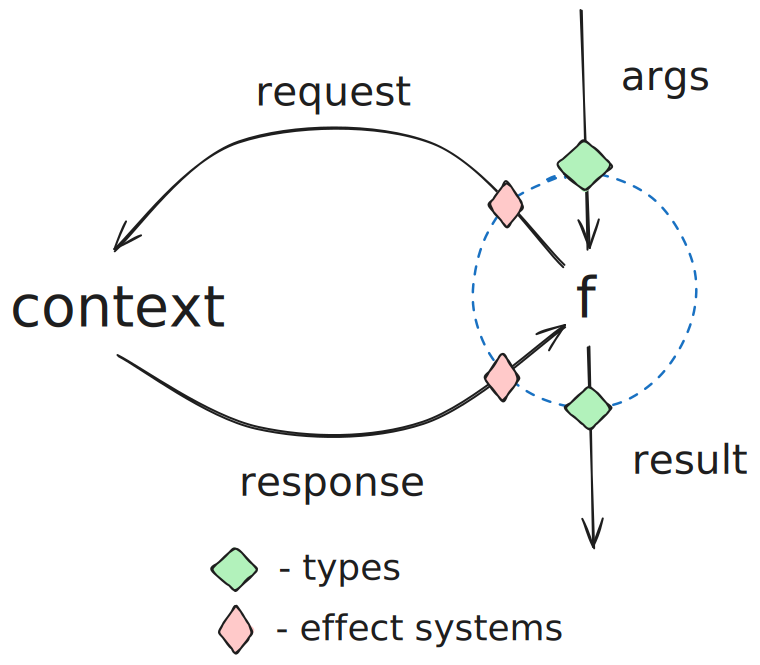
\includegraphics[width=\textwidth]{figs/context-communication}
                \end{center}
            \end{column}
        \end{columns}
    \end{frame}

    \begin{frame}[fragile]{Why do we need effect systems}
        \begin{itemize}
            \item[1.] Clarify abstraction borders --- all \emph{observable} context dependencies of functions in types
            \item[2.] \pause Establish \vocab{effect safety} --- ensure that context actually supports such effects
            \item[\eg] Thrown exceptions should be eventually handled
            \item[\eg] Required service implementation is provided
            \item[3.] \pause Control \vocab{effect encapsulation (abstraction)} --- no effects are handled accidentally\footnote{Lindley, Sam. "Encapsulating effects." \textit{Dagstuhl Reports, Volume 8, Issue 4}. 2018.}
            \item[\eg] Higher-order function can eventually handle exception from parameter function
            \begin{minted}{kotlin}
                fun withContent(path: String, f: (String) -> Unit) =
                    try {
                        val content = readFromFile(path)
                        f(content) // can accidentally catch exception from here
                        deleteFile(path)
                    } catch (e: FileException) {}
            \end{minted}
            \item Certainty by construction software
        \end{itemize}
    \end{frame}

    \begin{frame}[fragile]{Free variables are the essence}
        \vspace{-1em}
        \begin{columns}[onlytextwidth]
            \begin{column}{0.485\textwidth}
                \begin{itemize}
                    \item[\defi] \textbf{Free variables} --- variables that are not defined in a particular computation
                    \item So their meaning depend on the context (code around)
                    \item[\NB] An effect system is about managing free variables
                    \item Free variables can be dynamically or lexically scoped\ldots
                \end{itemize}
            \end{column}\hfill%
            \begin{column}{0.485\textwidth}
                \begin{minted}{swift}
                    func f(x: Int64) {
                        op(x) // `op` is free for `f`
                        let g = { =>
                            x + 1 // `x` is free for ?$\lambda$?
                        }
                        g
                    }
                \end{minted}
            \end{column}
        \end{columns}
    \end{frame}

    \sectionplan{Row-based effect systems}

    \begin{frame}[fragile]{Row-based effect systems with row-polymorphism}
        \begin{itemize}
            \item \emph{All} function effects are represented as an unordered row of labels
            \[\Lambda a\ldotp\lambda xs\ldotp map \ap (\lambda x\ldotp print\ap x; yield\ap x) \ap xs : \forall a \ldotp list\ap a \to^{\{print, yield \ap a\}} list \ap unit \]
            \item Need to use \vocab{effect polymorphism} to inherit effects of fist-class functions
            \[printMap = \Lambda \mu \ap a \ap b\ldotp \lambda f\ap xs\ldotp \ldots : \forall \mu \ap a \ap b\ldotp (a \to^\mu b) \to list \ap a \to^{\{print|\mu\}} list \ap b \]
            \item There is a subtyping relation on effect rows
            \item[\NB] Need to annotate all HOFs --- verbose, cannot introduce effect checking incrementally
            \item Effect safety is ``obvious''
        \end{itemize}
    \end{frame}

    \begin{frame}[fragile]{Duplicated labels and effect encapsulation\footnote{``Koka: Programming with row-polymorphic effect types'', D.Leijen, 2014.}}
        \begin{itemize}
            \item Labels can duplicate: $\{exc, exc\} \neq \{exc\}$
            \item Helps for type inference determinism ($\{exc|\mu\} \sim \{exc\} \rightsquigarrow \mu = \{\}$)
            \item Otherwise \texttt{catch} will be supposed to deal with all exceptions
            \[catch : \forall \mu\ap a\ldotp (unit\to^{\{exn|\mu\}} a, exception \to^{\mu} a) \to^\mu a\]
            \item Duplication provides effect encapsulation
            \begin{gather*}
                inject : \forall\mu a\ldotp (()\to^{\{exn|\mu\}}a) \to^{\{exn,exn|\mu\}} a
                \\
                \lambda x\ldotp catch(\ldots;~\underbrace{inject(\lambda \_\ldotp throw)}_{\{exn,exn\}};~\ldots, \lambda\_\ldotp x) : a \to^{exn} a
            \end{gather*}
            \item[\NB] Row-based system support, but do not force encapsulation
        \end{itemize}
    \end{frame}

    \sectionplan{Capability-based effect systems}

    \begin{frame}[fragile]{Dynamically scoped free variables}
        \vspace{-1em}
        \begin{columns}[onlytextwidth]
            \begin{column}{0.485\textwidth}
                \begin{itemize}
                    \item[\defi] Computation use site determines the meaning of such variables
                    \item Implicit parameters is a close approximation in static languages
                \end{itemize}
            \end{column}\hfill%
            \begin{column}{0.485\textwidth}
                \begin{minted}{swift}
                    context(op: (Int64) -> Unit)
                    func f(x: Int64) {
                        ...
                    }

                    context let op = ...
                    f(12) // `op` is passed implicitly
                \end{minted}
            \end{column}
        \end{columns}
    \end{frame}

    \begin{frame}[fragile]{Dynamically scoped variables as context validity witnesses}
        \vspace{-1em}
        \begin{columns}[onlytextwidth]
            \begin{column}[]{0.485\textwidth}
                \begin{itemize}
                    \item We require a call site to pass witness arguments (\textbf{capabilities}) of special types to proof its validity
                    \item A function's effects become explicit
                    \item Context is guaranteed to be appropriate
                    \item[\eg] Exception handlers are witnessed by parameters of magic \texttt{Handler} type
                    \item[\NB] Reason about effects just as about bindings --- implicits represent context requirements
                \end{itemize}
            \end{column}\hfill%
            \begin{column}[]{0.485\textwidth}
                \begin{minted}{swift}
                    context(
                        config: Config,
                        send: (...) -> Unit,
                        SomeException
                        // h: Handler<SomeException>
                    )
                    func f() {
                        send(config.address, ...)
                        if (...) {
                            throw SomeException() // to h
                        }
                    }
                \end{minted}
            \end{column}
        \end{columns}
    \end{frame}

    \begin{frame}[fragile]{Example: Kotlin context parameters\footnote{\color{blue}\url{https://github.com/Kotlin/KEEP/blob/context-parameters/proposals/context-parameters.md}}}
        \begin{itemize}
            \item Can define a capability and it's scope
            \begin{minted}{kotlin}
                class FileError {
                    fun reportNotFound(fileName: String): Nothing = throw FNFE(fileName)
                }
                fun <R> withFileError(block: context(FileError) () -> R) =
                    try {
                        with (FileError()) { block() }
                    } catch (e: FileNotFoundException) { println(e) }
            \end{minted}
            \item Capabilities are passed implicitly by type
            \begin{minted}{kotlin}
                context(fe: FileError)
                fun workWithFiles() = fe.reportNotFound("text.txt")

                withFileError {
                    workWithFiles()
                }
            \end{minted}
        \end{itemize}
    \end{frame}

    \begin{frame}[fragile]{Lexically scoped free variables}
        \vspace{-1em}
        \begin{columns}[onlytextwidth]
            \begin{column}[]{0.485\textwidth}
                \begin{itemize}
                    \item[\defi] Computation definition side determines the meaning
                    \item[\eg] Closure capturing
                \end{itemize}
            \end{column}\hfill%
            \begin{column}[]{0.485\textwidth}
                \begin{minted}{swift}
                    func f(x: Int64) {
                        let g = { =>
                            x + 1 // lexically scoped
                        }
                        g
                    }

                    let g = f(1)
                    let x = 42
                    g() // returns 2
                \end{minted}
            \end{column}
        \end{columns}
    \end{frame}

    \begin{frame}[fragile]{Contextual polymorphism}
        \begin{itemize}
            \item Lexical scoping helps with higher-order functions
            \item Can avoid using effect polymorphism in many cases
        \end{itemize}
        \vspace{1em}
        \begin{minted}[escapeinside=##]{swift}
            func map<T, R>(xs: List<T>, f: (T) -> R): List<R>

            context(config: Config, send: (...) -> String, SomeException)
            func testMap() {
                let results = map([1, 2]) { x =>
                    #\framebox{send}#(#\framebox{config}#.endpoint, x)
                    if (...) throw SomeException() // to #\framebox{h}#
                }
                printAll(results)
            }
        \end{minted}
    \end{frame}

    \begin{frame}[fragile]{Effect encapsulation works by default}
        \begin{minted}{swift}
            func withSomeException<R>(f: context(SomeException) () -> R): R {
                try { // h1: Handler<SomeException>, h2: Handler<AnotherException> =>
                    f() // {h1}
                } catch (e: SomeException) {
                    ...
                } catch (e: AnotherException) {
                    ... // unreachable code
                }
            }

            withSomeException { context(SomeException) =>
                if (...) throw SomeException()
                else throw AnotherException() // captured
            }
        \end{minted}
    \end{frame}

    \begin{frame}[fragile]{Effect system safety}
        \vspace{-1em}
        \begin{columns}[onlytextwidth]
            \begin{column}[]{0.485\textwidth}
                \begin{itemize}
                    \item Capabilities proof context validity
                    \item Capabilities should not leak the scope they were provided to
                    \item Need escape analysis to control this\ldots
                \end{itemize}
            \end{column}\hfill%
            \begin{column}[]{0.485\textwidth}
                \begin{minted}[escapeinside=##]{swift}
                    var f: () -> Unit = {}
                    try { // h =>
                        f = {
                            throw SomeException() // to #\framebox{h}#
                        }
                    } catch (e: SomeException) {...}
                    f() // boom
                \end{minted}
            \end{column}
        \end{columns}
    \end{frame}

%    \begin{frame}[fragile]{Example: context parameters}
%        \begin{itemize}
%            \item Context parameters are \emph{not safe}
%            \begin{minted}{kotlin}
%                fun crash() {
%                    lateinit var leak: FileError
%                    withFileError {
%                        leak = implicit<FileError>()
%                    }
%                    leak.reportNotFound("out of scope")
%                }
%            \end{minted}
%            \item Context parameters do not guarantee effect abstraction (can be intentionally introduced)
%            \begin{minted}{kotlin}
%                fun accidentalHandling(block: () -> Unit) =
%                    try {
%                        doMyJob1(); block(); doMyJob2()
%                    } catch (e: FileNotFoundException) {
%                        println("I'm not supposed to catch things from block")
%                    }
%            \end{minted}
%        \end{itemize}
%    \end{frame}

    \begin{frame}[fragile]{Type-based escape analysis for effect safety\footnote{``Gentrification Gone too Far? Affordable 2nd-Class Values for Fun and (Co-)Effect'', Osvald et al, 2016.}}
        \begin{block}{Rules}
            \begin{enumerate}
                \item Capabilities are second-class
                \item First-class functions cannot refer to second-class values through free variables
                \item Functions can return only first-class values
                \item Only first-class values can be stored in object fields or mutable variables
            \end{enumerate}
        \end{block}
        \begin{itemize}
            \item[\eg]
            \begin{minted}{kotlin}
                fun <R> withFile(f: @local (@local File) -> R): R
                withFile { newFile -> { oldFile.copyTo(newFile) } } // error
            \end{minted}
            \item Or just make all functions second-class --- \vocab{blocks}\footnote{``Effects as Capabilities: Effect Handlers and Lightweight Effect Polymorphism'', Brachthäuser et al, 2020.}
            \begin{minted}{scala}
                def foreach[A](l: List[A]) { f: A => Unit }: Unit
            \end{minted}
            \item[\NB] We cannot even write curried \texttt{map}!
            \item[\NB] Everything is very bad with OOP staff as well
        \end{itemize}
    \end{frame}

    \begin{frame}[fragile]{``From Scope-Based Reasoning to Type-Based Reasoning and Back''\footnote{``Effects, Capabilities, and Boxes'', Brachthäuser et al, 2022.}}
        \begin{itemize}
            \item Want to restore first-class-ness for functions
            \item Implicitly track in context for each variable over which capabilities it closes
            %! suppress = EscapeAmpersand
            \begin{align*}
                \infer[Tracked]{\Gamma\vdash f : \sigma ~|~ \{f\}}{f :^\star \sigma \in \Gamma}
                &&
                \infer[Transparent]{\Gamma\vdash f : \sigma ~|~ C}{f :^C \sigma \in \Gamma}
            \end{align*}
            \item Boxing: add information about capabilities from context to types
            \begin{align*}
                \infer[BoxIntro]{\Gamma \vdash \mathbf{box}\ap b : \sigma~ \mathbf{at}\ap C ~|~ \{\}}{\Gamma \vdash b : \sigma ~|~ C}
                &&
                \infer[BoxElim]{\Gamma \vdash \mathbf{unbox}\ap e : \sigma ~|~ C}{\Gamma \vdash e : \sigma ~\mathbf{at}~C ~|~ \{\}}
            \end{align*}
            \item Boxed blocks are first-class values, unboxing checks capabilities
            \item Using \vocab{reference-dependent types} for effect polymorphism
            \begin{minted}{haskell}
                fun <T, R> map(f: (T) -> R): (List<T>) -> R at {f} = box { xs -> go(f, xs) }
                map { x -> console.print(x) } : (List<T>) -> Unit at {console}
            \end{minted}
        \end{itemize}
    \end{frame}

    \begin{frame}[fragile]{Effekt --- language with implicit capabilities\footnote{\color{blue}\url{https://effekt-lang.org/}}}
        \begin{itemize}
            \item Capabilities provide effectful signatures readings
            \begin{minted}[escapeinside=##]{scala}
                def buildString(ident : Int)
                  { f : Unit => Unit / {Emit[String]} } : String / {Format}
                //                   #\big\uparrow# capabilities to be provided by buildString
                //          capabilities required by buildString #\big\uparrow#
            \end{minted}
            \item Effect encapsulation enabled by default --- can provide only explicitly declared capabilities
            \begin{minted}{scala}
                def encapsulated { f : Unit => Unit / {} } : Unit =
                  try { ...; f(); ... } with Exn { ... }
            \end{minted}
            \item Uses boxing and reference-dependent effect polymorphism tracking effect tags
            \begin{minted}{scala}
                def map[T, R] { f : T => R } : List[T] => List[R] at {f}
                map { x => do print(x); x + 1 } : List[T] => List[R] at {Console}
            \end{minted}
            \item Anonymous objects are second-class by default like functions
            \item Type inference is mostly future work
        \end{itemize}
    \end{frame}

    \begin{frame}[fragile]{Scala scoped capabilities\footnote{``Scoped capabilities for polymorphic effects'', Odersky et al, 2022..}\footnote{\color{blue}\url{https://docs.scala-lang.org/scala3/reference/experimental/cc.html}}}
        \begin{itemize}
            \item Every value can be marked as tracked (or capability) in type-level: \mintinline{scala}|File^|
            \item Values enumerate captured capabilities in types by names: \mintinline{scala}|LazyList[Int]^{file,f}|
            \item Object capability set --- capabilities saved in class primary constructor
            \item Capabilities form a hierarchy
            \begin{minted}{scala}
                def usingLogFile[T](f: OutputStream^, op: (Logger^{f}) => T): T =
                  op(Logger(f))
            \end{minted}
            \item \mintinline{scala}|->| --- pure function, \mintinline{scala}|=>| --- tracked function (\mintinline{scala}|->^|), \mintinline{scala}|->^{c1,c2}| --- capturing c1 and c2
        \end{itemize}
    \end{frame}

    \begin{frame}[fragile]{Scala capture checking example}
        \begin{minted}[escapeinside=##]{scala}
            class FileSystem

            class Logger(fs: FileSystem^):
              def log(s: String): Unit = ??? // Write to a log file, using `fs`

            def test(fs: FileSystem^): LazyList[Int]^{fs} =
              val l: Logger^{fs} = Logger(fs)
              l.log("hello world!")
              val xs: LazyList[Int]^{l} =
                LazyList.from(1)
                  .map { i =>
                    l.log(s"computing elem # $i")
                    i * i
                  }
              xs
        \end{minted}
    \end{frame}

    \sectionplan{Modal-based effect systems}

    \begin{frame}[fragile]{Modal effect types\footnote{``Modal Effect Types'', Sam Lindley et al, 2024.}}
        \begin{itemize}
            \item Modal logic is about different models of truth: must be true, may be true\ldots
            \item Type modalities tell about usability of type in different contexts
            \item Insight: types should mark transitions between effect contexts, rather than repeating context
            \item Modalities are boxes describing context they can be unboxed in
            \item Modalities inference is similar to first-class polymorphism
            \item[\NB] Everything is first-class, you pay transferring context borders
            \item Formalizing Frank's abilities\footnote{``Doo bee doo bee doo'', Lucas Convert et al.}
        \end{itemize}
    \end{frame}

    \begin{frame}[fragile]{Absolute modalities}
        \begin{itemize}
            \item Describes full effect context
            \begin{minted}{haskell}
                gen : [yield](List Int -> 1)
                gen xs = map (fun x -> do yield x); ()
            \end{minted}
            \item Function with only described effects
            \begin{minted}{haskell}
                asList : [yield](1 -> 1) -> List Int
                asList m = handle m () with
                  return () -> []
                  yield x r -> x :: r ()
            \end{minted}
            \item Boxes are first-class, can be stored in data structures
            \item Unboxing is implicit (can be prevented with tilde), boxing --- explicit
            \begin{minted}{haskell}
                asList [yield](fun () -> yield 1; yield 2; ())
            \end{minted}
            \item Paper do not describe polymorphic modalities
            \begin{minted}{haskell}
                asList : [yield e](1 -> 1) -> List e
            \end{minted}
        \end{itemize}
    \end{frame}

    \begin{frame}[fragile]{Relative modalities}
        \begin{itemize}
            \item Define effect transformations: bring me to the right context and I'll unbox
            \begin{minted}{haskell}
                --       #\big\downarrow# can use all effects of the context plus `yield`
                asList : <yield>(1 -> 1) -> List Int
                asList m = handle m () with ...
                --                #\big\uparrow# transfered value to right context
            \end{minted}
            \item Variable should be used only under the context compatible with binding occurrence
            \item Effect encapsulation:
            \begin{minted}{haskell}
                find : (Int -> Bool) -> List Int -> Maybe Int
                find p xs = handle
                  (map (fun x -> if mask(p x) then do yield x else ()) xs) with ...
            \end{minted}
            \item Relative modalities are enough to type functions with at most one row-polymorphic variable
            \item Cannot encode curried map, need effect polymorphism
            \begin{minted}{haskell}
                map : [e](a -> b) -> [e](List a -> List b)
            \end{minted}
            \item There is a kind system allowing some types freely pass context boundaries
        \end{itemize}
    \end{frame}

    \sectionplan{Summary}

    \begin{frame}[fragile]{Summary about effect systems}
        \begin{itemize}
            \item Effect systems are about tracking free variables
        \end{itemize}
        \begin{block}{Dynamically scoped free variables}
            \begin{itemize}
                \item Dealt by implicits
                \item Represent unfulfilled context requirements of a computation
                \item User specifies more function parameters
            \end{itemize}
        \end{block}
        \begin{block}{Lexically scoped free variables}
            \begin{itemize}
                \item Dealt by type-based escape analysis
                \item Represent fulfilled context requirements of a computation
                \item User specifies a function's dataflow
            \end{itemize}
        \end{block}
    \end{frame}

    \begin{frame}[fragile]{Relation to other approaches}
        \begin{block}{Canonical row-polymorphic effect systems (a la Koka)}
            \begin{itemize}
                \item Tracks only dynamically scoped free variables
                \item We use coeffect-style instead (use left side of a turnstile)
            \end{itemize}
        \end{block}
        \begin{block}{Capability-based effect systems (a la Scala, Effekt)}
            \begin{itemize}
                \item Uses implicits as well (or ``context readings'')
                \item Uses dependent typing to do escape analysis (lifetimes are values)
            \end{itemize}
        \end{block}
        \begin{block}{Modal effect types}
            \begin{itemize}
                \item Relative modalities a like unfulfilled implicits
                \item Lifetime information erased, every context boundary transition changes context requirements of a type
            \end{itemize}
        \end{block}
    \end{frame}

\end{document}
